\begin{figure*}
\center{
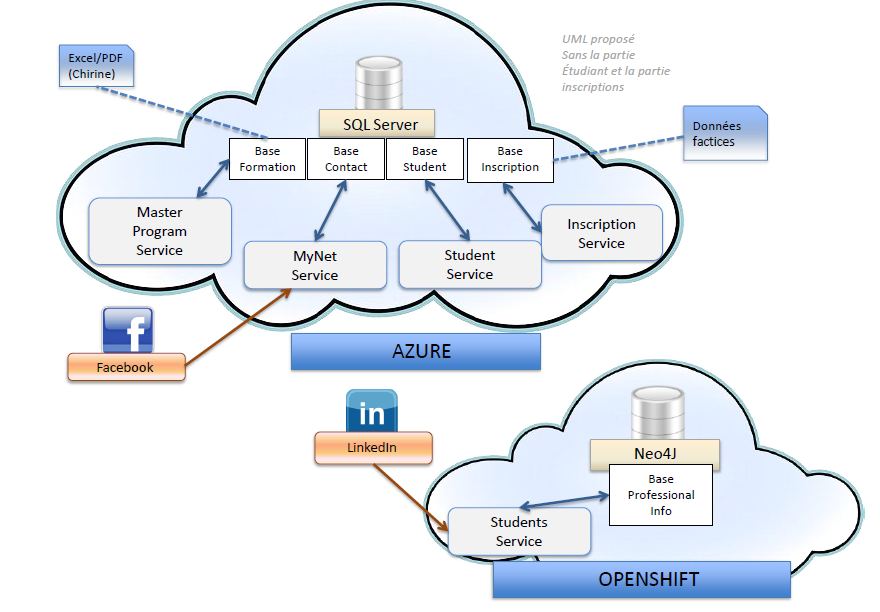
\includegraphics[width=0.65\textwidth]{use-case.png}
\caption{General distributed data storage service.\label{fig:storage}}}
\end{figure*}

According to our example scenario, we conducted an experimental experience for implementing our data integration approach on a multi-cloud environment. We focussed on the implementation of a data as a service layer that integrates content from different services related to education but also related on data producers and consumers. Figure \ref{fig:storage} shows the general architecture of our scenario, deployed on Window Azure data store services and on Jelastic (https://jelastic.com), an open free cloud provider where we installed NE4J and Mongo NoSQL stores. The multi-cloud data as a service layer is a data provision platform storing clean data sets stemming from public data services (Linked in, Tweeter, Facebook) accessible on Internet and also from private ones. 

The DaaS platform interacts recurrently with services in order to retrieve data and build collections that can be accessed by consumers. Each data service is characterized by the quality of data it provides, its availability and also by privacy and data ownership contrats provided as SLA contracts and enforced by security protocols.
